\documentclass[conference]{IEEEtran}
\IEEEoverridecommandlockouts
\usepackage{cite}
\usepackage{amsmath,amssymb,amsfonts}
\usepackage{algorithmic}
\usepackage{graphicx}
\usepackage{textcomp}
\usepackage{graphicx}
\graphicspath{ {./images/} }
\usepackage{xcolor}
\usepackage[utf8]{inputenc}
\usepackage{hyperref}
\usepackage{xcolor}
\usepackage{pgfplots}
\usepackage{listings}
\usepackage{multicol}
\usepackage{amsmath}
\def\BibTeX{{\rm B\kern-.05em{\sc i\kern-.025em b}\kern-.08em
    T\kern-.1667em\lower.7ex\hbox{E}\kern-.125emX}}

\begin{document}

\title{
Tracing sorted subsequence in a random matrix row-wise and column-wise \\
}

\author{\IEEEauthorblockN{Harsh Kedia}
\IEEEauthorblockA{IIB2019028}
\and
\IEEEauthorblockN{Milap Anwani}
\IEEEauthorblockA{IIB2019029}
\and
\IEEEauthorblockN{Kandagatla Meghana Santhoshi}
\IEEEauthorblockA{IIB2019030}
}

\maketitle

\noindent \begin{abstract}

In this paper ,we have devised an algorithm to trace all the sorted subsequences in a random matrix both row-wise and column-wise. We have used recursion to solve the problem and also analysed the time and space complexity of the program.\\\\
Keyword : Subsequence, Recursion, Time complexity, Space complexity.

\end{abstract}

\section{\textbf{Introduction}}
\noindent In this problem, we have to find all the sorted subsequences, by traversing through each row and each column. \\


\noindent For example, let's suppose the matrix is: \\\
0 2 \\
5 4 \\
Then all the sorted subsequences in the matrix are:\\\
 \{(2), (0), (4), (5), (0,2)\} \\
  
\noindent We will use recursion to solve the problem.\\

\noindent \textbf{Recursion} is the process in which a function calls itself directly or indirectly and the corresponding function is called as recursive function.\\
\noindent In the recursive program, the solution to the base case is provided and the solution of the bigger problem is expressed in terms of smaller problems.\\

\noindent The algorithm  is described in detail in \textbf{part II}.\\

\section{\textbf {Algorithm Description and Analysis}}

 Driver function:\\
\begin{enumerate}

\item We are  generating a random matrix in the main and is sent to driver function as input.\\

\item In driver function we are initialising a vector of int "ls1" as each row one by one is forwarded to find function to calculate the sorted sub sequences.\\

\item For each row after computation it is stored in 2D vector 'st'.
\\

\item To find column wise, we find store each column as rows in trans matrix and then similarly we compute sorted subsequences for each column in matrix or each row in trans matrix. \\

\item In this way we compute sorted subsequences for a matrix, row-wise and column-wise.\\

\end{enumerate}

 Find function: \\

\begin{enumerate}

\item In find function, if input row is empty and output row is not empty then, storing the result in 2D vector  "st" and return.\\

\item Else , initalise temp vector and push back value first element of row and erase that value from input row.\\

\item Call find function and if output row is empty then call it again with output row as temp.\\

\item Else if first element of temp is greater then last element of output row , then push back that temp value in output row.\\

\item Again call find function. \\

\end{enumerate}

\section{\textbf{Pseudo Code}}

\lstset { %
    language=C++,
    backgroundcolor=\color{black!6},
    basicstyle=\footnotesize,
}
2D vector st is used to store results after computation.find function has two vectors inp and out to store the current input and current output respectively in its prototype as we are using recursion.
\begin{lstlisting}

 Function driver :

	For : i - > 0 to R  
	   initialise vector<int>ls1
	   ls1=matrix[i]
	   Declare vector<int>ls2
       find(ls1,ls2)
       print st 
       clear st 
    
    For: i->0 to C
      For : j -> 0 to R
      transmatrix[i][j] = matrix[j][i];
      
    For : i - > 0 to C 
	   initialise vector<int>ls1
	   ls1=transmatrix[i]
	   Declare vector<int>ls2
       find(ls1,ls2)
       print st
       clear st 
        
Function find :
    
    if(inp.empty()&&out.size()!=0)
    st.push_back(out)
    else return
    
    intialise vector temp
    temp.push_back(inp[0])
    erase the first element in inp
    find(inp, out)
    
    if(out.size() == 0)
		find(inp, temp)
	
    else(temp[0] > out[out.size() - 1])
		out.push_back(temp[0])
		find(inp, out)


\end{lstlisting}

\section{\textbf {Time Complexity}}
\noindent The time complexity of finding subsequence in each row/column is O({$2^n$}) and thus time complexity of the whole program is O(n\cdot{$2^n$}).

\begin{figure}[htp]
    \centering
    \includegraphics[width=8cm]{TimeComplexity}
    \caption{Time complexity curve}
    \label{fig:timecomplexity.png}
\end{figure}

\section{\textbf {Auxiliary Space Complexity}}
\noindent The space complexity of the program is O({$n^2$}). This is because we are using matrices here.

\begin{figure}[htp]
    \centering
    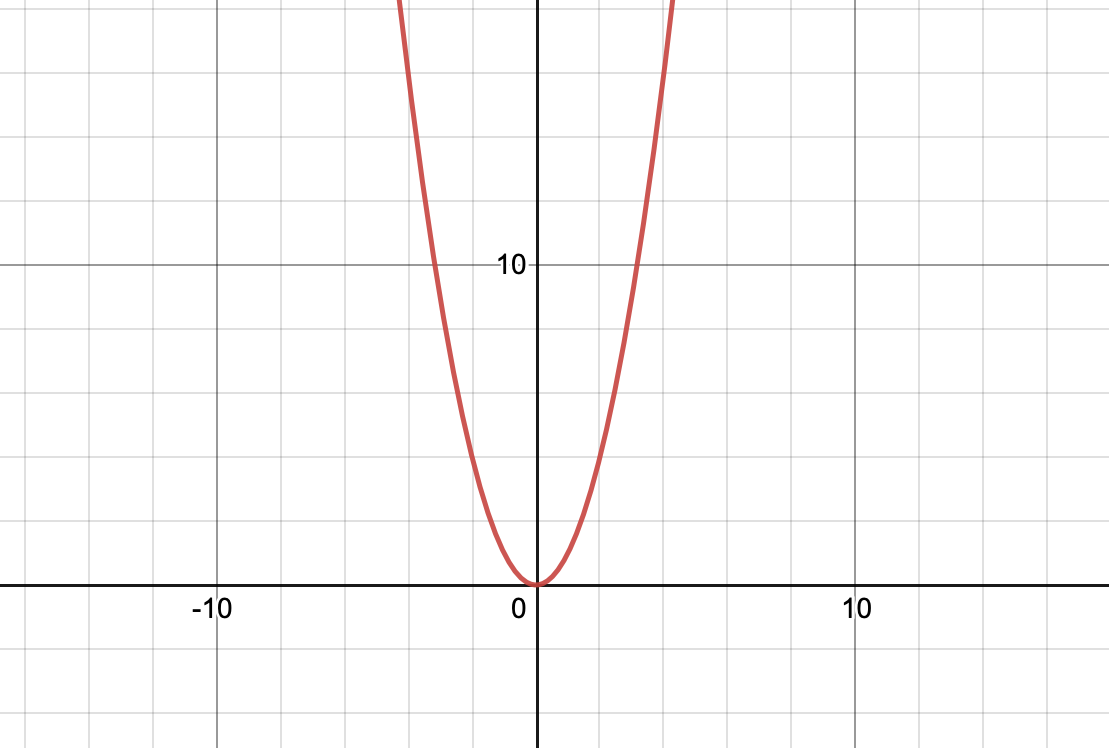
\includegraphics[width=8cm]{spacecomplexity}
    \caption{Space complexity curve}
    \label{fig:spacecomplexity.png}
\end{figure}

\section{\textbf {Conclusion}} \noindent We have arrived at the solution of the problem by recursion, where we are operating on each row and column, thus the time complexity is O(n\cdot{$2^n$}).\\

\section{Applications}
Recursion is a wide variety of algorithmic technique which believes on the strategy of calling the other problems and combine them.This methodology has many predefined algorithms which work on the basis of Recursion. Some of the applications of the Recusrion Approach are:

\begin{enumerate}
\item \textbf{DFS traversal of a graph}
\item \textbf{Tower of Hanoi problem}
\item \textbf{Tree traversals like inorder,postorder and preorder} 
\item \textbf{ All Backtracking algorithms are based on recursion} etc many more.

\end{enumerate}

\section{\textbf{Acknowledgment}}
We are very much grateful to our Course instructor Mr.Rahul kala and Dr.Javed  and our mentor, Mr.Md Meraz, who have provided the great opportunity to do this wonderful work on the subject of Data Structure and Algorithm Analysis.

\section{\textbf {References}} 

We have referred [3] to clear the basic concepts of Recursion.Reference [2] helped us , to develop solution of this question.[1] helped us to generate random matrix.
\begin{thebibliography}{00}
\bibitem{b1}https://www.codespeedy.com/generate-a-matrix-of-random-numbers-in-cpp/
\bibitem{b2}https://www.geeksforgeeks.org/number-of-longest-increasing-subsequences/
\bibitem{b3}https://www.inf.unibz.it/~calvanese/teaching/06-07-ip/lecture-notes/uni11.pdf

\end{thebibliography}

\section{\textbf{Appendix}}

\subsection{Project link on Github:}
https://github.com/maggi2k19/DaaAssignments/Assignment - 06

\end{document}
\end{document}
